\chapter{Case Study}
\label{ch:case}
% INTRODUCTION
% concise introduction to the chapter, its goals, and structure.
In this chapter, we discuss the case study we conducted in order to validate our prototype tool, ScriptButler. The goal of a case study is to demonstrate that the functionality of our tool actually answers our research questions. We previously verified our tool in Section \ref{sec:testing} and in this chapter, we validate it. 

We first describe the game we chose for our game study, what kind of game it is, what kind of features it has and why it is useful for our purpose. We then explain the methodology we use when conducting our case study and what kind of results we expect. We explain what the results are designed to show. Finally, we describe our actual results, reflect on them and discuss how they prove the validity of the tool.

The reason that we do this case study on an existing game rather than designing our own specifically for a case study is that we do not have game designers as part of the project team. This means that any game we created would not be created by the target audience of the prototype tool. 


% The chapter is broken down as follows:
% \begin{itemize}
%     \item We describe the game we selected for the case study, what kind of features it has, how it works and why we selected it.
%     \item We describe the methodology that we use when conducting our case study and what kind of results we expect. We also describe what our results are designed to show.
%     \item Finally we describe our results, reflect on them and discuss how they prove the validity of our tool.
%     \item 
% \end{itemize}

\section{Methodology}
% describe the measurements and tests, and what they are designed to show.
Our case study is based on the following hypothesis:\newline
\quad \textit{"If we remove specific parts of the code then the game should still compile and run but the gameplay should \emph{break}."}

\textit{Break} is defined as issues indirectly caused by the removal of certain code. For example, removing a game mechanic that allows players to push a crate has the direct effect of making it impossible for the player to push a crate. However, it also has the indirect effect of making levels where pushing crates is required impossible to solve. This is because removing code also has a direct effect on gameplay and how the player can interact with the game, functionality is related to gameplay. 

Game designers create their game iteratively, as such, code is bound to be removed and added as the software evolves. We simulate this iterative by removing code from the game based on the impact it will have and observing how the tool reacts. We create three modified versions of the game, each of the modification change a single line of code but creates a large impact on the gameplay. The modifications are all listed in Table \ref{fig:case_study_experiment} and explained below.

% each version has a small modification, an expected goal and an objective. The objective is meant to describe what we expect the result to prove as far as validation goes. The three modifications, their expect results and objectives can be seen in Figure \ref{fig:case_study_experiment} and explained below.

Please note that we do not test our prototype tool on the published version of the game but on our own modified version, even in the case when we test on an "unmodified" version. This modified version includes additional newlines and the removal of redundant white space so as to make it simpler for our prototype grammar to parse it efficiently. Line numbers used in this chapter all reference lines in our modified versions which can be found on the repository of the project\footnote{\url{https://github.com/ClementJ18/ScriptButler/tree/main/src/PuzzleScript/Test/Case}}

% Our first modification is the removal of line 210, which is the win condition that states that no object Objective must be present. 

The first modification removes the win condition, which states that no object must be present (line 210). As previously explained this is intended to be the first part of every level, with the second part being the return to the Exit objects. The Win Conditions are one of the three main parts of a game where software evolution can have heavy indirect consequences. The other two that we will be testing in this case study are Game Mechanics (Rules) and Level Layouts (Levels).

Modifying win conditions changes how the player interacts with the levels, large parts of the intended player routes are made optional, changing the difficulty rating and obstacles that the player faces. The error messages that appear are used to make sure the game designer realizes that so that they can take the appropriate steps. In this case, the appropriate state, given that the removal of the win condition is intended, is to restructure the level so that the player needs to avoid guards to reach the exit.

\begin{figure}[!t]
    \centering
    \caption{Experimental setup}
    \begin{tabular}{p{4cm}|p{11cm}}
    \textbf{Action} & \textbf{Expected Results} \\ \hline
    Remove the "No Objective" win condition & Tool should raise errors due to levels that can be completed without user interaction or by going in a single direction \\ \hline
    Remove rule \#2 & Tool should raise errors stating that a win condition is impossible because there is no way to get meet it given that it is not already fulfilled on a level \\ \hline
    Remove Exit objects from levels & Tool should raise an error stating the level is impossible because there is no way to get from the current level set up to a level setup that meets the win conditions \\ \hline
    \end{tabular}
    \label{fig:case_study_experiment_old}
\end{figure}

% The second modification is the removal of the rule on line 193, this rule allows the player to remove the Objective object, fulfilling the requirement of "No Objective".

The second modification is the removal on the rule that allows the player to remove the Objective object (line 193). This rule is the mechanic that allows players to satisfy the "No Object" win condition. Removing the rule should remove the mechanic and therefore make it impossible to satisfy the condition. Theoretically, this should only apply to levels where there is an Objective present to remove but in the case of this game, it is every level. Even in the case where it doesn't actually apply to any level the tool assumes that win conditions are intended to be fulfilled on at least one level. If that is not the case, then another error is raised stating the condition is already fulfilled, which alerts the game designer to the problem. This modification relates to how the change in source code changes game mechanics and impact player interaction.

The third modification we perform is the removal of all Exit objects from certain levels, hence making these levels impossible to solve because of the evolution of level layouts. When level layouts evolve it sometimes causes the level to become unwinnable or to simply become too easy to win. Because the game only has two victory conditions and one of them is a negation we can only check this by removing the Exit objects. Removing other objects will have either no effect or will cause pathfinding issues which our prototype tool does not check for.

All three modifications are extreme cases of software evolution, the case in which something is removed. These cases are meant to illustrate how iterative design can render break gameplay or render it redundant and how meta-programming tools can help solve the problem. The results of the experiments are error and warning messages generated by our prototype and attached directly to the IDE at the appropriate line.

\section{Timothy's Adventure}
% describe the case of Timothy's adventure. What is the game and how does it work.
The game we are studying, Timothy's Adventure has a simple concept. Steal the shiny objective, avoid the guards and escape. You cannot escape until you have stolen the shiny objective.

The victory conditions are expressed in two lines, that state the objective must have been removed and that the player must be on the "exit" tiles. The narrative of this game is that the player is some sort of thief who must grab some shiny object (represented as the objective) and exit the room (by being on the exit objects). As with most PuzzleScript games, a lot of its mechanics and defeat/victory conditions are implied and must be discovered by the user, usually either through the use of common design choices or through messages at the beginning of the level.

For this case study, we extracted the exact win conditions and game mechanics by observing the code. There are five key mechanics defined by about a dozen rules. The first is tied to the \textit{Objective} Win Condition, it states that if a player is near an Objective object and presses the action key it replaces it with another object, removing that specific Objective from being an obstacle for the condition. The next two mechanics relate to the defeat condition of the game. PuzzleScript does not provide the ability to create defeat conditions the same way it provides for victory conditions. By default, the defeat condition is a softlock, an event that happens when player interaction reaches a level state that cannot become a level state that meets the conditions even if the player can still alter the level. Sometimes, as with this particular game, the designers create explicit defeat conditions with rules that automatically restart the level if the player reaches a certain state. Two mechanics take care of this defeat condition, the first one states that if a Guard object is on the same X or Y axis as the Player object then they will move one block in the player's direction and the second states that if a Guard is adjacent to the Player object then the Player object is replaced with another object representing that the player got "caught" and then the level restart at the next loop.

\begin{figure}[!t]
    \centering
    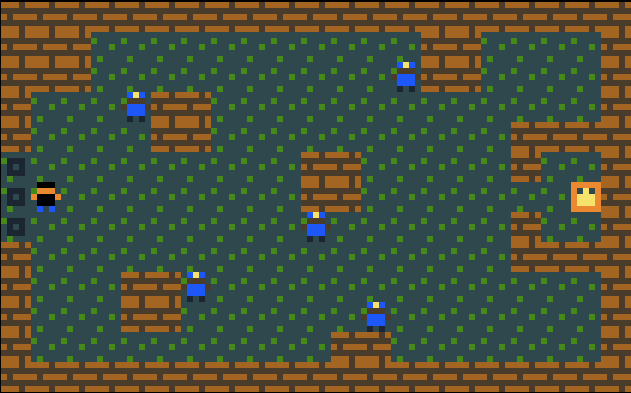
\includegraphics[width=0.75\textwidth]{images/case_results/Case_game.png}
    \caption{A level from the case game showcasing the general layout with the exit on the left, the objective on the right and the guards in blue}
    \label{fig:case_game_example_old}
\end{figure}

Finally, the game has two mechanics which represent tools that the players can use to solve certain levels. The first mechanic, introduced in level 5, allows the player to step on a Button object which transforms every Door object on the same X and Y axis into a different object which neither the player nor the guards can go through. This is usually used to stop guards from getting to the player but can also softlock the player if used without care. The second mechanic and the most complex one of the game is related to movement. It states that if the player steps on a Portal object then they will be teleported to the equivalent portal object on the same X or Y axis given that it is not obstructed. This is used to allow the player to move to rooms that are not connected to one another or to escape guards as they cannot use the portal.

% There are five game mechanics expressed in about a dozen rules:
% \begin{itemize}
%     \item Pressing action next to the switch flips it
%     \item Being on the same X or Y axis as a guard makes them move towards you
%     \item Being adjacent to a guard on the start of the turn makes you lose the level
%     \item Stepping on a button activates all the walls on the same X or Y coordinate
%     \item Stepping on a portal sends you to a portal if one exists unobstructed on the same X or Y coordinate
% \end{itemize}

The game contains 14 levels, each of them created with the goal of gradually increasing the difficulty by introducing new challenges and new mechanics to solve those challenges. 

\section{Results}
% you describe the experimental results, and you reflect on them.
Here we validate ScriptButler in a case study of the game called Timothy's adventure.
% Without modifications, our prototype tool raises the following errors and warnings, by order of appearance:

We first run the tool on an unmodified version of the game to see what errors or warnings may already exist and find the following issues, by order of appearance:
\begin{itemize}
    \item WARNING: Line 33 - Color \textbf{white} not used in object Background 4
    \item WARNING: Line 161 - Legend \textbf{ + } defined but not used
    \item WARNING: Line 199 - Right side of rule similar to rule on line 200
    \item WARNING: Line 200 - Right side of rule similar to rule on line 199
    \item ERROR: Line 202 - Objects in section need to be able to stack but appear on the same layer.
\end{itemize}

We first want to address the error, a false positive as a result of a misinterpretation of PuzzleScript's design. The side of the rule with the error is \texttt{Background no Wall no Door\_on}, which the checker interprets as meaning that the three items specified should be able to stack when in fact what this line actually means is that there should be no wall or door present on this background.

There is an argument to be made there that this is an unnecessary ambiguity since when objects are aligned in a part of the rule it usually means that they should be able to stack. In addition, there are already tools that can avoid this sort of ambiguity by creating an extra \textbf{or} reference that include both, as can be seen in Figure \ref{fig:case_ambiguity}

\begin{figure}[!t]
\begin{lstlisting}[language=PuzzleScript]
Obstacle = Wall or Door_on
[> Temp Teleport | Background no Obstacle] -> [ Teleport > Player_stealth | Background]
\end{lstlisting}
\vspace*{-8pt}
\caption{Removing design ambiguity from the rule}
\label{fig:case_ambiguity_old}
\vspace*{-8pt}
\end{figure}

The remaining warnings are all valid but not critical as they are mainly dead code or intended false positives that inform designers about potential issues with gameplay.

\subsection{Modifying Victory Conditions}
\textit{Remove the ”No Objective” win condition}

The results of the modification matched our expectations, removing the win conditions labelled all the levels are trivially solvable by going in a single direction. This modification theoretically matches our idea of rapid feedback but, in practice, our prototype implementation cannot identify trivial solutions fast enough to be considered rapid feedback. This is caused by optimization issues with the engine and not with the dynamic analyser, as such, optimization work on the engine will easily resolve our issue with performance in the dynamic analysis. A sample of the warning messages generated next to the levels can be seen in Figure \ref{fig:modification_1_results}

\begin{figure}[!t]
    \centering
    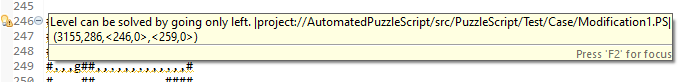
\includegraphics[width=1\textwidth]{images/case_results/Modification_1_Results.png}
    \caption{Warning messages are shown after applying modification 1}
    \label{fig:modification_1_results_old}
\end{figure}

\subsection{Modifying Game Mechanics}
\textit{Remove rule \#2}

The result of the modification matched our expectations, removing the first rule triggered a warning stating that the win condition "No Objective" is now impossible to fulfil, given that it is not already fulfilled on a level. The tool assumed by default that every rule and every win condition is used on every level, this means that some of the messages are false but those can simply be ignored by the game designer. Guessing whether or not a rule is intended to be used by the game designer could lead to a lot of false negatives. We prefer having some false positives that the designer can ignore rather than false negatives that they may never find out about.

The error message can be seen in Figure \ref{fig:modification_2_results}, it is located on the same line as the problematic win condition although it does hide it when hovered as can be seen on this screenshot. As a reminder, our tool does not conduct any pathfinding analysis as this is more of an AI-focused goal. We assume that the player is able to reach the necessary objects for victory and focus on whether or not they are able to interact with them in a way that could lead to a solution. 

\begin{figure}[!t]
    \centering
    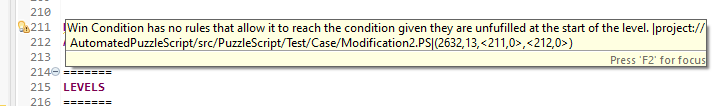
\includegraphics[width=1\textwidth]{images/case_results/Modification_2_Results.png}
    \caption{A warning message is shown after applying modification 2}
    \label{fig:modification_2_results_old}
\end{figure}

\subsection{Modifying Level Layouts}
\textit{Remove Exit objects from levels}

This case study was trickier than we initially intended. Player objects have special rules attached to them related to their movement and as such the tool needs to be specifically told that the object has those special rules. The rest is simple enough, analyse if the object is present on the map, if it is not, analyse if there is a way to spawn it. Because of the special rules we do not need to perform this analysis on the players, our assumption is that at least one player object is always present 

For every condition not already met on a level, we check if it can be met specifically within the context of this level. As with others, this can lead to false positives, especially with complex levels in which conditions only become an obstacle to victory after a prerequisite has been met. Although these cases are rare as this usually means that this prerequisite has to be filled anyways in order to reach the condition. 

\begin{figure}[!t]
    \centering
    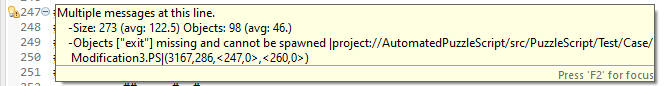
\includegraphics[width=1\textwidth]{images/case_results/Modification_3_Results.png}
    \caption{A warning message is shown after applying modification 3}
    \label{fig:modification_3_results_old}
\end{figure}

\begin{figure}[!t]
\begin{lstlisting}[language=PuzzleScript]
(BEFORE)
###########
#....O....#
#.........#
#.........#
#.........#
#....P....#
####EEE####

(AFTER)
###########
#....O....#
#.........#
#.........#
#.........#
#....P....#
####...####
\end{lstlisting}
\vspace*{-8pt}
\caption{Removing exit objects from level}
\label{fig:case_m3_modification_old}
\vspace*{-8pt}
\end{figure}

We validated this check by temporarily adding a rule to the modification that would allow the player to spawn an exit. This successfully erased all error messages relating to that issue.

\section{Conclusion}
In our case study, we set out to show that the error and warning messages that ScriptButler raises are indeed related to the software evolution in games and that the tool can indeed tell the game designer when their code changes impact the gameplay in a negative manner. 

We use simple examples to answer our hypothesis since these simple examples can easily be confirmed by playing the game manually to validate them. Therefore, since we know that our examples are valid cases of software evolution impacting gameplay in a negative way, we can validate our tool by having the tool raise warnings on the cases.

It accomplishes the goal for all three of the modifications from which we can then extrapolate, with a small degree of incertitude related to validity threats (discussed in Section \ref{sec:threats}), that our tool could accomplish the same with more complex cases of software evolution having an impact on gameplay. 

% \section{Threats to validity}
% % What could affect the validity of your research? Think of pitfalls of your research method, experimental setup, interpreting the results.

% Our prototype tool does suffer from a few issues but the core of it is functional. The two main threats to the validity of our results is performance and feature-completion.

% We, however, not do perceive these as critical threats to the validity of our research. We have proven that we are able to implement a bit of everything that PuzzleScript offers and we have found no reason to believe that the rest would be impossible to implement. Making the engine feature complete will be complex but not impossible. 

% Performance is a more complicated issue. A large part of the performance issue comes from an initially shaky understanding of PuzzleScript's design. Our understanding became more solid as the project progressed which allowed us to fix some of the issues. The first step to fixing performance would most likely make the tool feature complete first once the every part of the implementation is done it would be easier to understand how to rework the code to make it more optimal.



